\documentclass{article}
\usepackage{layout}
\usepackage[utf8]{inputenc}
\usepackage[a4paper, total={6in, 8in}]{geometry}
\usepackage{graphics}
\usepackage{amsmath}


\graphicspath{ {./src/} }


\headheight=0pt
\title{\textbf{Kinematic calculations for mobile robots using Omni/Meccanum wheels}}
\author{Sujith Christopher}
\date{January 2023}
\begin{document}

\maketitle

\section{Generalized expression}

% refer book
\begin{large}
    This general expression is taken from the book
    "Modern robotics mecanics planning and control" by Kevin M Lynch, Frank C Park,
    page no 512, please refer this section for more details.
\end{large}


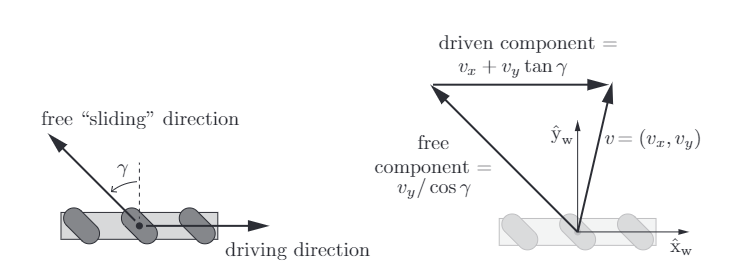
\includegraphics{omni_wheel_kinematics_2.png}


\section{Three wheel omnidirectional robot}
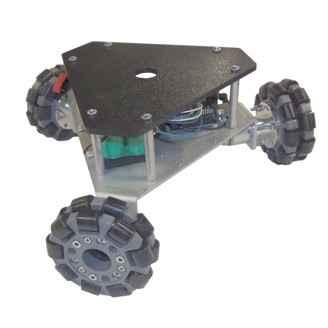
\includegraphics{robot_3_omniwheel.jpg}


\begin{equation}
    h_1(0) \mathcal{V}_b = \frac{1}{r_i} \left[\begin{array}{cc}
            1 & \tan\gamma_i \\
        \end{array}\right]
    \left[\begin{array}{cc}
            \cos \beta_i  & \sin \beta_i \\
            -\sin \beta_i & \cos \beta_i \\
        \end{array}\right]
    \begin{bmatrix}
        -y_i & 1 & 0 \\
        x_i  & 0 & 1 \\
    \end{bmatrix} \mathcal{V}_b
\end{equation}

\begin{equation}
    \gamma_1 = 0, \beta_1 = 0
\end{equation}

\begin{equation}
    = \frac{1}{r_1} \left[\begin{array}{cc}
            1 & 0 \\
        \end{array}\right]
    \left[\begin{array}{cc}
            \cos 0  & \sin 0 \\
            -\sin 0 & \cos 0 \\
        \end{array}\right]
    \begin{bmatrix}
        -y_1 & 1 & 0 \\
        x_1  & 0 & 1 \\
    \end{bmatrix}
    \mathcal{V}_b
\end{equation}

\begin{equation}
    = \frac{1}{r_1} \left[\begin{array}{cc}
            1 & 0 \\
        \end{array}\right]
    \left[
        \begin{array}{cc}
            1 & 0 \\
            0 & 1 \\
        \end{array}\right]
    \begin{bmatrix}
        -y_1 & 1 & 0 \\
        x_1  & 0 & 1 \\
    \end{bmatrix}
    \mathcal{V}_b
\end{equation}
\begin{equation}
    = \frac{1}{r_1}
    \left[
        \begin{array}{cc}
            1 & 0 \\
        \end{array}\right]
    \mathcal{V}_b
\end{equation}

\begin{equation}
    r_i = r_1 = r_2 = r_3 = r
\end{equation}

\begin{equation}
    h_1(0) \mathcal{V}_b = \frac{1}{r}
    \left[
        \begin{array}{cc}
            1 & 0 \\
        \end{array}\right]
    \mathcal{V}_b
\end{equation}

% new page
\newpage
\section{Four wheel omnidirectional robot}




\end{document}